\documentclass[11pt,a4paper]{article}
\usepackage[margin=2.5cm,headheight=15pt]{geometry}
\usepackage{amsmath,amssymb,amsthm}
\usepackage{mathtools}
\usepackage{microtype}
\usepackage{hyperref}
\usepackage{cleveref}
\usepackage{enumitem}
\usepackage{mdframed}
\usepackage{xcolor}
\usepackage{titlesec}
\usepackage{booktabs}
\usepackage{tikz}
\usetikzlibrary{positioning,arrows.meta,shapes.geometric,calc}
\usepackage{fancyhdr}

\definecolor{navyblue}{RGB}{26,58,92}
\definecolor{midblue}{RGB}{44,95,138}
\definecolor{lightblue}{RGB}{232,240,248}
\definecolor{proofgray}{RGB}{242,242,242}
\definecolor{warncolor}{RGB}{255,245,220}
\definecolor{warnborder}{RGB}{180,100,0}
\definecolor{opencolor}{RGB}{235,245,235}
\definecolor{openborder}{RGB}{0,120,0}

\hypersetup{colorlinks=true,linkcolor=midblue,citecolor=midblue,urlcolor=midblue}

\pagestyle{fancy}\fancyhf{}
\fancyhead[L]{\small\color{navyblue}\textit{JGP+GSP Heuristic: Gap Analysis and Bounds}}
\fancyhead[R]{\small\color{navyblue}\thepage}
\renewcommand{\headrulewidth}{0.4pt}

\titleformat{\section}{\large\bfseries\color{navyblue}}{}{0em}{}[\color{navyblue}\titlerule]
\titleformat{\subsection}{\normalsize\bfseries\color{midblue}}{}{0em}{}
\titleformat{\subsubsection}{\normalsize\itshape\color{midblue}}{}{0em}{}

\newmdenv[backgroundcolor=lightblue,linecolor=navyblue,linewidth=1.2pt,
  leftline=true,rightline=false,topline=false,bottomline=false,
  innerleftmargin=12pt,innerrightmargin=8pt,innertopmargin=8pt,
  innerbottommargin=8pt,skipabove=10pt,skipbelow=6pt]{thmbox}

\newmdenv[backgroundcolor=proofgray,linecolor=midblue,linewidth=0.8pt,
  leftline=true,rightline=false,topline=false,bottomline=false,
  innerleftmargin=10pt,innerrightmargin=8pt,innertopmargin=6pt,
  innerbottommargin=6pt,skipabove=6pt,skipbelow=6pt]{proofbox}

\newmdenv[backgroundcolor=warncolor,linecolor=warnborder,linewidth=1.2pt,
  leftline=true,rightline=false,topline=false,bottomline=false,
  innerleftmargin=12pt,innerrightmargin=8pt,innertopmargin=8pt,
  innerbottommargin=8pt,skipabove=10pt,skipbelow=6pt]{warnbox}

\newmdenv[backgroundcolor=opencolor,linecolor=openborder,linewidth=1.2pt,
  leftline=true,rightline=false,topline=false,bottomline=false,
  innerleftmargin=12pt,innerrightmargin=8pt,innertopmargin=8pt,
  innerbottommargin=8pt,skipabove=10pt,skipbelow=6pt]{openproblem}

\theoremstyle{plain}
\newtheorem{theorem}{Theorem}[section]
\newtheorem{lemma}[theorem]{Lemma}
\newtheorem{proposition}[theorem]{Proposition}
\newtheorem{corollary}[theorem]{Corollary}
\newtheorem{conjecture}[theorem]{Conjecture}
\theoremstyle{definition}
\newtheorem{definition}[theorem]{Definition}
\newtheorem{remark}[theorem]{Remark}
\newtheorem{example}[theorem]{Example}
\newtheorem{question}[theorem]{Open Question}

\DeclareMathOperator{\OPT}{OPT}
\newcommand{\Kstar}{K^{*}}
\newcommand{\ZJGP}{Z_{\mathrm{JGP}}^{*}}
\newcommand{\ZSSP}{Z_{\mathrm{SSP}}^{*}}
\newcommand{\Tunion}{\bigl|\bigcup_{j} T_j\bigr|}

\setlist[itemize]{noitemsep,topsep=4pt}
\setlist[enumerate]{noitemsep,topsep=4pt}

% =============================================================================
\begin{document}
% =============================================================================

\begin{center}
  {\color{navyblue}\rule{\textwidth}{2pt}}\\[0.4cm]
  {\LARGE\bfseries\color{navyblue}The Job Sequencing and Tool Switching Problem}\\[0.3cm]
  {\large\itshape\color{midblue}Part V: JGP\,+\,GSP Heuristic --- Gap Analysis and Bounds}\\[0.2cm]
  {\color{navyblue}\rule{\textwidth}{2pt}}
\end{center}

\begin{mdframed}[backgroundcolor=lightblue,linecolor=navyblue,linewidth=1pt,
  innerleftmargin=14pt,innerrightmargin=14pt,innertopmargin=8pt,innerbottommargin=8pt]
\small\textbf{Scope and status.}
This note studies the additive gap $\mathrm{gap}(I)=H(I)-\ZSSP(I)$ and the ratio
$H(I)/\ZSSP(I)$ between the cost $H$ of the two-phase \emph{JGP\,+\,GSP} heuristic
and the optimal uniform-SSP cost $\ZSSP$. What is \textbf{proved} here:
(i)~two lower bounds on $\ZSSP$ --- the grouping bound $\ZSSP\ge\Kstar-1$ and the
tool-counting bound $\ZSSP\ge\bigl|\bigcup_jT_j\bigr|-b$ (\cref{thm:lb_k,thm:lb_tools}),
together with the classical $\ZSSP\le b(\Kstar-1)$;
(ii)~a computationally certified counterexample (the $6$-job ring) with
$\mathrm{gap}=1$ and ratio $4/3$ (\cref{ex:ring});
(iii)~a construction with $\mathrm{gap}=g$ for every $g$, so the gap is
\emph{unbounded} (\cref{thm:unbounded});
(iv)~a directly computable gap bound $\mathrm{gap}\le H-\max(\Kstar-1,\,|\bigcup_jT_j|-b)$
(\cref{prop:gapbound}) and two sufficient conditions for zero gap (\cref{thm:suffA,thm:suffB});
(v)~a \emph{grouping-exactness} theorem (\cref{thm:grouping_exact}): $\ZSSP$ equals the
minimum GTSP cost over \emph{all} feasible groupings, so the gap is exactly the price of
using the fewest groups, and a sub-optimal grouping can strictly beat the heuristic
(\cref{thm:subopt}).
What is \textbf{conjectural}: the tight ratio bound $H/\ZSSP\le 4/3$ for $b=3$
(\cref{conj:ratio}); it is \emph{not} proved, and the previously attempted route
via $\sum_kR_k\le H/4$ is false and is retracted (\cref{rem:retract}).
All numerical assertions are verified by the scripts in
\texttt{plans-genai/\_verification/} (see \texttt{VERIFIED\_FACTS.md}); reproduce with
\texttt{python3 run\_study.py}.
\end{mdframed}

\vspace{0.4cm}
\tableofcontents
\newpage

% =============================================================================
\section{The JGP\,+\,GSP Heuristic}
\label{sec:heuristic}
% =============================================================================

We work throughout with the \emph{uniform} SSP: a single magazine of capacity $b$,
jobs $j\in J$ with required tool sets $T_j\subseteq T$, $|T_j|\le b$, and switch cost
equal to the number of tool insertions along the processed sequence. We adopt the
\emph{free-initial-load} convention: the first $\le b$ tools are loaded for free
(equivalently, the sequence starts from a free dummy depot), so $\ZSSP$ counts only
the insertions made between consecutive jobs. For a fixed sequence the optimal loading
is computed by KTNS \cite{Tang1988}.

\subsection{The Job Grouping Problem (JGP)}

\begin{definition}[Feasible group]
A set of jobs $G\subseteq J$ is \emph{feasible} if all its tools fit simultaneously:
$\bigl|\bigcup_{j\in G}T_j\bigr|\le b$.
\end{definition}

\begin{definition}[JGP as set covering/partitioning \cite{Crama1994,Catanzaro2015}]
Let $\mathcal{S}$ be the family of feasible groups and $y_G\in\{0,1\}$. The JGP is
\[
  \ZJGP=\min\Bigl\{\textstyle\sum_{G\in\mathcal{S}}y_G:\
  \sum_{G\ni j}y_G\ge 1\ \ \forall j\in J,\ y_G\in\{0,1\}\Bigr\},
\]
the minimum number of feasible groups (``batches'') that cover $J$. We write
$\Kstar=\ZJGP$.
\end{definition}

\begin{remark}[Hardness and exact solution]
The JGP is NP-hard \cite{Crama1994}. It is solved exactly by the ARF MILP of
Catanzaro et al.\ \cite{Catanzaro2015} and by Branch-and-Price \cite{Otiai2024}; the
pricing subproblem generates maximal feasible groups (a set-union knapsack).
\end{remark}

\begin{warnbox}
\textbf{Feasibility is a group property, not a pairwise one.}
A group is feasible iff the union of \emph{all} its tool sets fits in $b$. This is
stronger than pairwise compatibility: the three jobs $\{t_1,t_2\},\{t_1,t_3\},\{t_1,t_4\}$
($b=3$) are pairwise compatible (each pairwise union has size $3$) yet jointly infeasible
($|\{t_1,t_2,t_3,t_4\}|=4>b$). Consequently $\Kstar$ is \emph{not} in general the
chromatic number of the pairwise conflict graph; see \cref{sec:conflict}.
\end{warnbox}

\subsection{From Groups to Configurations and the GSP}

Given a grouping $G_1,\dots,G_K$, each group $G_k$ must be served by a
\emph{configuration} $C_k$ (a magazine state with $|C_k|=b$) that covers it.

\begin{definition}[Configuration cluster and slack]
For a group $G$ with required set $T^{(G)}=\bigcup_{j\in G}T_j$,
\[
  \mathcal{C}(G)=\bigl\{C\subseteq T:\ |C|=b,\ T^{(G)}\subseteq C\bigr\},
  \qquad s(G)=b-|T^{(G)}|\ge 0 .
\]
The $s(G)$ free slots (``slack'') may be filled with tools of \emph{adjacent} groups
to lower the transition cost.
\end{definition}

\begin{definition}[Group Sequencing Problem and the heuristic cost $H$]
\label{def:heuristic}
The \emph{GSP} chooses, for a given grouping, a permutation $\pi$ of the groups and a
configuration $C_k\in\mathcal{C}(G_k)$ for each $k$, minimising
\[
  H(\pi,\{C_k\})=\sum_{i=1}^{K-1}\bigl|C_{\pi(i+1)}\setminus C_{\pi(i)}\bigr|
  =\sum_{i=1}^{K-1}\bigl(b-|C_{\pi(i)}\cap C_{\pi(i+1)}|\bigr).
\]
This is a path \textbf{Generalised TSP} over the clusters $\{\mathcal{C}(G_k)\}$. The
JGP\,+\,GSP \emph{heuristic} (1) solves the JGP to get a $\Kstar$-grouping, then
(2)~solves the GSP exactly; its cost is
\[
  H \;=\; \min_{\text{JGP-optimal groupings}}\ \min_{\pi,\{C_k\}} H(\pi,\{C_k\}),
\]
the minimum over all $\Kstar$-group JGP solutions of the GTSP optimum. Any such schedule
is a feasible SSP solution, so $H\ge\ZSSP$.
\end{definition}

\begin{thmbox}
\begin{lemma}[Per-transition lower bound]
\label{lem:transition}
For an ordered adjacent pair $G_k,G_{k+1}$, every choice of configurations costs at least
\[
  w^{*}(G_k,G_{k+1})=\max\!\Bigl(0,\ \bigl|T^{(G_k)}\cup T^{(G_{k+1})}\bigr|-b\Bigr).
\]
For \emph{zero-slack} groups ($s(G_k)=s(G_{k+1})=0$) the configurations are forced
($C_k=T^{(G_k)}$) and the transition costs exactly $b-|T^{(G_k)}\cap T^{(G_{k+1})}|$.
\end{lemma}
\end{thmbox}

\begin{proofbox}
\begin{proof}
$C_{k+1}\supseteq T^{(G_{k+1})}$ has $s(G_{k+1})$ free slots; of the
$|T^{(G_k)}\setminus T^{(G_{k+1})}|$ tools that $C_k$ holds but $G_{k+1}$ does not
require, at most $s(G_{k+1})$ can be retained, so at least
$\max(0,|T^{(G_k)}\setminus T^{(G_{k+1})}|-s(G_{k+1}))=\max(0,|T^{(G_k)}\cup T^{(G_{k+1})}|-b)$
must leave. With zero slack no tool can be retained beyond the required set, giving the
stated exact cost.
\end{proof}
\end{proofbox}

\begin{warnbox}
\textbf{Greedy ``lookahead'' is not globally optimal for the GSP.}
Filling each group's slack with the next group's tools (lookahead) attains the
per-transition bound of \cref{lem:transition} for one isolated transition, but the
padding of $C_k$ influences \emph{both} the $(k\!-\!1,k)$ and $(k,k\!+\!1)$ transitions,
so summing per-transition minima can under-count. The true heuristic cost $H$ is the
GTSP optimum of \cref{def:heuristic}, which we compute exactly. For \emph{zero-slack}
instances there is no padding freedom and the GSP reduces to a TSP over forced
configurations; all worst-case instances in this note are zero-slack, where the per-transition
formula is exact.
\end{warnbox}

% =============================================================================
\section{Lower and Upper Bounds Relating $\ZSSP$, $\Kstar$ and the Tool Count}
\label{sec:bounds}
% =============================================================================

Two elementary but distinct lower bounds control $\ZSSP$. Both are used repeatedly.

\begin{thmbox}
\begin{theorem}[Grouping lower bound \cite{Crama1994}]
\label{thm:lb_k}
$\ZSSP\ge \Kstar-1.$
\end{theorem}
\end{thmbox}
\begin{proofbox}
\begin{proof}
An optimal SSP solution visits a sequence of magazine states; let $W_1,\dots,W_m$ be the
distinct states in order of first appearance. Each job is served by some $W_r$, so
$\{W_1,\dots,W_m\}$ covers $J$ by feasible configurations and $m\ge\Kstar$. Consecutive
distinct states differ in $\ge 1$ tool, so the number of insertions is $\ge m-1\ge\Kstar-1$.
\end{proof}
\end{proofbox}

\begin{thmbox}
\begin{theorem}[Tool-counting lower bound]
\label{thm:lb_tools}
Let $U=\bigcup_{j\in J}T_j$. Then $\ZSSP\ge |U|-b.$
\end{theorem}
\end{thmbox}
\begin{proofbox}
\begin{proof}
Every tool of $U$ is required by some job, hence is loaded into the magazine at least
once. At most $b$ tools occupy the initial free load; every other loading is a counted
insertion. Therefore the number of insertions is at least $|U|-b$.
\end{proof}
\end{proofbox}

\begin{remark}[Relation to the SSPMF bound]
\label{rem:msc}
$|U|-b$ is exactly the $M-C$ linear-programming lower bound of the multicommodity-flow
formulation (SSPMF) of da Silva et al.\ \cite{daSilva2024} ($M=|U|$ tools, $C=b$ capacity);
\cref{thm:lb_tools} gives the elementary combinatorial proof. Combining the two bounds,
\[
  \boxed{\ \ZSSP\ \ge\ \max\bigl(\Kstar-1,\ |U|-b\bigr).\ }
\]
\end{remark}

\begin{thmbox}
\begin{theorem}[Grouping upper bound \cite{Crama1994}]
\label{thm:ub}
$\ZSSP\le b\,(\Kstar-1).$
\end{theorem}
\end{thmbox}
\begin{proofbox}
\begin{proof}
Process a $\Kstar$-group JGP solution batch by batch under one fixed covering
configuration per batch. The initial load is free; each of the $\Kstar-1$ inter-batch
transitions inserts at most $b$ tools.
\end{proof}
\end{proofbox}

\begin{warnbox}
\textbf{Which bound is tight?}
Neither lower bound is tight in general, and their maximum need not equal $\ZSSP$.
On the ring family of \cref{sec:counterexample} and on the entire exhaustively
enumerated $b=3$ edge family (jobs $=$ graph edges, $|T_j|=2$; $10691$ instances)
we verified $\ZSSP=\max(\Kstar-1,|U|-b)$ with no exception. But this equality is
\emph{family-specific}: among $b=3$ instances with $|T_j|\le 3$ on $\le5$ tools,
$2410$ of $21569$ have $\ZSSP$ strictly above \emph{both} bounds, and the $b=4$
sliding window $T_{j_i}=\{i,i{+}1,i{+}2\}\bmod 8$ has $\ZSSP=5>\max(3,4)$. Only the
inequality of \cref{rem:msc} is universal.
\end{warnbox}

% =============================================================================
\section{A Certified Counterexample: the $6$-Job Ring}
\label{sec:counterexample}
% =============================================================================

\begin{example}[$6$-job ring]
\label{ex:ring}
Let $T=\{t_1,\dots,t_6\}$, $b=3$, and
$T_{j_i}=\{t_i,t_{i+1\bmod 6}\}$ for $i=1,\dots,6$: consecutive jobs share one tool.

\smallskip\noindent\textbf{JGP optimum ($\Kstar=3$).} The minimum number of feasible
groups is $3$ (two optimal groupings exist). One is
$G_1=\{j_1,j_2\},\,G_2=\{j_3,j_4\},\,G_3=\{j_5,j_6\}$ with required sets
$T^{(1)}=\{t_1,t_2,t_3\}$, $T^{(2)}=\{t_3,t_4,t_5\}$, $T^{(3)}=\{t_1,t_5,t_6\}$, each of
size $3$ (zero slack), so configurations are forced.

\smallskip\noindent\textbf{JGP\,+\,GSP cost ($H=4$).} With forced configurations the GSP
is a TSP on three nodes; every pair of the three sets shares exactly one tool, so each
transition costs $b-1=2$ and any order pays $2\times2=4$. Thus $H=4$.

\smallskip\noindent\textbf{SSP optimum ($\ZSSP=3$).} The sequence
$j_1\to\cdots\to j_6$ under KTNS:
\begin{center}
\begin{tabular}{lccc}
\toprule
Step & Job & Magazine & Switches \\
\midrule
1 & $j_1$ & $\{t_1,t_2,t_3\}$ & (free initial load) \\
2 & $j_2$ & $\{t_1,t_2,t_3\}$ & 0 \\
3 & $j_3$ & $\{t_1,t_3,t_4\}$ & 1 \ ($-t_2,+t_4$) \\
4 & $j_4$ & $\{t_1,t_4,t_5\}$ & 1 \ ($-t_3,+t_5$) \\
5 & $j_5$ & $\{t_1,t_5,t_6\}$ & 1 \ ($-t_4,+t_6$) \\
6 & $j_6$ & $\{t_1,t_5,t_6\}$ & 0 \\
\bottomrule
\end{tabular}
\end{center}
KTNS retains $t_1$ as a \emph{bridge} across jobs $j_2$--$j_5$, so $\ZSSP=3$, matching
both lower bounds: $|U|-b=6-3=3$ (and $\Kstar-1=2$).

\smallskip\noindent\textbf{Gap.} $H-\ZSSP=4-3=1$; ratio $4/3$. Verified exactly by
state-DP and by PORTA enumeration.
\end{example}

\begin{figure}[h!]
\centering
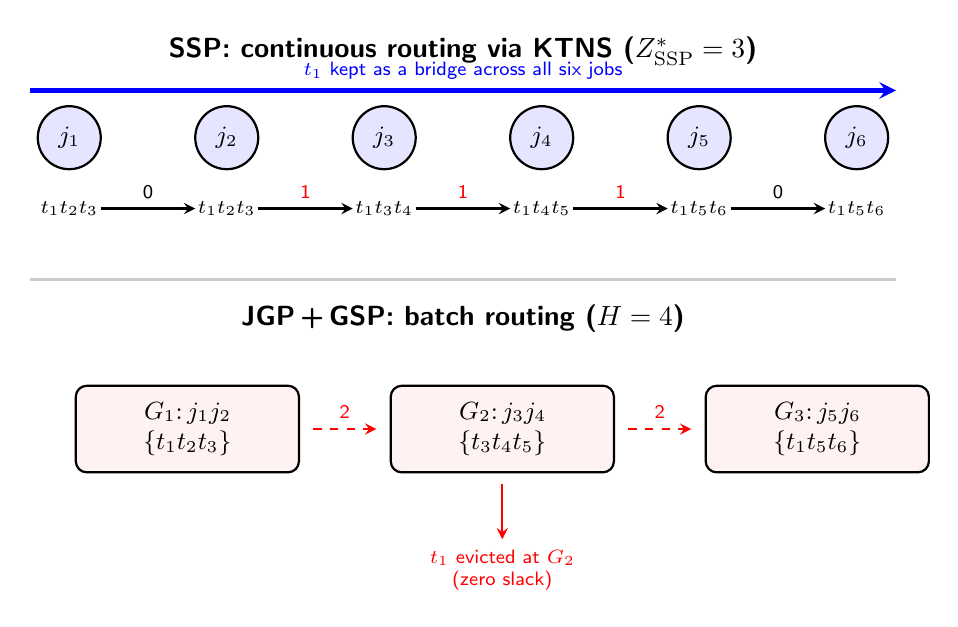
\begin{tikzpicture}[>=stealth]
  \tikzset{
    job/.style={circle,draw=black,thick,fill=blue!10,minimum size=0.8cm,font=\sffamily\small},
    conf/.style={rectangle,draw=black,thick,fill=red!5,text width=2.6cm,align=center,
                 rounded corners,minimum height=1.1cm,font=\sffamily\small},
    arr/.style={->,thick,black}, stop/.style={->,thick,dashed,red}}
  \node[font=\sffamily\bfseries] at (5,4.5){SSP: continuous routing via KTNS ($\ZSSP=3$)};
  \foreach \x/\lb in {0/$j_1$,2/$j_2$,4/$j_3$,6/$j_4$,8/$j_5$,10/$j_6$}
    \node[job] at (\x,3.4){\lb};
  \foreach \x/\mag in {0/{$t_1t_2t_3$},2/{$t_1t_2t_3$},4/{$t_1t_3t_4$},6/{$t_1t_4t_5$},
     8/{$t_1t_5t_6$},10/{$t_1t_5t_6$}}
    \node[font=\sffamily\scriptsize] at (\x,2.5){\mag};
  \draw[arr](0.4,2.5)--(1.6,2.5)node[midway,above,font=\sffamily\scriptsize]{0};
  \draw[arr](2.4,2.5)--(3.6,2.5)node[midway,above,font=\sffamily\scriptsize,red]{1};
  \draw[arr](4.4,2.5)--(5.6,2.5)node[midway,above,font=\sffamily\scriptsize,red]{1};
  \draw[arr](6.4,2.5)--(7.6,2.5)node[midway,above,font=\sffamily\scriptsize,red]{1};
  \draw[arr](8.4,2.5)--(9.6,2.5)node[midway,above,font=\sffamily\scriptsize]{0};
  \draw[ultra thick,blue,->](-0.5,4.0)--(10.5,4.0)
    node[midway,above,font=\sffamily\scriptsize]{$t_1$ kept as a bridge across all six jobs};
  \draw[thick,gray!40](-0.5,1.6)--(10.5,1.6);
  \node[font=\sffamily\bfseries] at (5,1.1){JGP\,+\,GSP: batch routing ($H=4$)};
  \node[conf]at(1.5,-0.3){$G_1{:}\,j_1j_2$\\$\{t_1t_2t_3\}$};
  \node[conf]at(5.5,-0.3){$G_2{:}\,j_3j_4$\\$\{t_3t_4t_5\}$};
  \node[conf]at(9.5,-0.3){$G_3{:}\,j_5j_6$\\$\{t_1t_5t_6\}$};
  \draw[stop](3.1,-0.3)--(3.9,-0.3)node[midway,above,font=\sffamily\scriptsize]{2};
  \draw[stop](7.1,-0.3)--(7.9,-0.3)node[midway,above,font=\sffamily\scriptsize]{2};
  \draw[->,thick,red](5.5,-1.0)--(5.5,-1.7)
    node[below,font=\sffamily\scriptsize,align=center]{$t_1$ evicted at $G_2$\\(zero slack)};
\end{tikzpicture}
\caption{The $6$-ring. KTNS keeps $t_1$ resident through all jobs ($3$ switches).
The $3$-group JGP saturates each batch with its required tools, forcing $t_1$ out at
$G_2$ and back in at $G_3$ ($4$ switches). Gap $=1$.}
\label{fig:ring}
\end{figure}

% =============================================================================
\section{The Gap is Unbounded}
\label{sec:gap_growth}
% =============================================================================

\begin{thmbox}
\begin{theorem}[Gap grows with $\Kstar$]
\label{thm:unbounded}
For every integer $g\ge 1$ there is a uniform-SSP instance with $\Kstar=3g$ on which the
JGP\,+\,GSP heuristic costs exactly $g$ more switches than the optimum:
$\ZSSP=6g-3$, $H=7g-3$, $\mathrm{gap}=g$.
\end{theorem}
\end{thmbox}
\begin{proofbox}
\begin{proof}
Take $g$ tool-disjoint copies of the $6$-ring (\cref{ex:ring}); copy $\ell$ uses tools
$\{t_{6\ell-5},\dots,t_{6\ell}\}$, so $|U|=6g$.

\emph{Optimum.} By \cref{thm:lb_tools}, $\ZSSP\ge|U|-b=6g-3$. Processing the copies
contiguously achieves this value (within a copy, $3$ switches as in \cref{ex:ring};
between two copies the magazine swaps completely, costing $b=3$, of which the first such
load per copy realises that copy's tool count); the explicit schedule attains $6g-3$, so
$\ZSSP=6g-3$.

\emph{Heuristic.} The clusters of different copies are tool-disjoint, so every
inter-copy transition costs $b=3$ and the GTSP decomposes: $H=\sum_{\ell}H^{(\ell)}+b(g-1)
=4g+3(g-1)=7g-3$.

Hence $\mathrm{gap}=H-\ZSSP=(7g-3)-(6g-3)=g$.
\end{proof}
\end{proofbox}

\begin{remark}[The gap scales with $\Kstar$, not $b$]
Here $\mathrm{gap}=g=\Kstar/3$, consistent with the worst-case envelope
$\mathrm{gap}\le H\le b(\Kstar-1)$ from \cref{thm:ub}. The relevant complexity
parameter for the additive gap is the number of groups $\Kstar$, not the capacity $b$.
The ratio, by contrast, \emph{shrinks} as $g$ grows: $(7g-3)/(6g-3)$ decreases from
$4/3$ at $g=1$ to $7/6$ as $g\to\infty$ (\cref{sec:ratio}). All values verified for
$g=1,\dots,4$.
\end{remark}

\begin{remark}[Two informal ``sources'' of gap]
\label{rem:sources}
It is tempting to split the gap into a \emph{padding} part (even the best configurations
for a fixed $\Kstar$-grouping cost more than $\ZSSP$) and a \emph{grouping} part (the SSP
optimum need not respect any $\Kstar$-grouping). This is a useful intuition but not a
theorem: the two effects are not independent and there is no proved decomposition. In the
$6$-ring, exhaustive enumeration of all $18$ feasible groupings shows the minimum GTSP
cost over $\Kstar$-groupings is $4$ while over \emph{all} groupings it is $3$; thus for
this instance the entire heuristic gap is removed by changing the grouping, not the
padding --- see \cref{thm:subopt}.
\end{remark}

% =============================================================================
\section{A Computable Gap Bound, the Bridge Mechanism, and the Ratio}
\label{sec:ratio}
% =============================================================================

\subsection{A directly computable gap bound}

\begin{thmbox}
\begin{proposition}[Gap bound]
\label{prop:gapbound}
For every instance,
\[
  0\ \le\ \mathrm{gap}(I)=H-\ZSSP\ \le\ H-\max\bigl(\Kstar-1,\ |U|-b\bigr).
\]
\end{proposition}
\end{thmbox}
\begin{proofbox}
\begin{proof}
$H\ge\ZSSP$ because the heuristic schedule is SSP-feasible; the upper bound substitutes
the proved lower bound $\ZSSP\ge\max(\Kstar-1,|U|-b)$ (\cref{rem:msc}).
\end{proof}
\end{proofbox}

\noindent For the $6$-ring this gives $\mathrm{gap}\le 4-\max(2,3)=1$, which is tight.
The bound is computable without solving the SSP, since $H$, $\Kstar$ and $|U|$ are all
available from the heuristic.

\subsection{The bridge / re-entry mechanism}

The gap is caused by tools the SSP keeps resident across a group boundary but the
heuristic must evict and reload.

\begin{definition}[Bridge tool]
\label{def:bridge}
Fix a $\Kstar$-grouping in GSP-optimal order. A tool $t$ is a \emph{bridge} if it is
required in some group $G_k$ and again in some later $G_{k'}$ ($k'>k$) but not required by
an intermediate group whose forced configuration must therefore evict it. KTNS can keep
$t$ resident through the intermediate jobs using slack, saving one insertion that the
heuristic pays.
\end{definition}

In the $6$-ring, $t_1$ is required by $j_1\in G_1$ and $j_6\in G_3$ but not by
$G_2=\{j_3,j_4\}$ (whose forced configuration is $\{t_3,t_4,t_5\}$). KTNS keeps $t_1$
through $j_2,\dots,j_5$; the heuristic evicts it at the $G_1\!\to\!G_2$ boundary and
reloads it at $G_2\!\to\!G_3$, which is the one extra switch.

\begin{warnbox}
\textbf{Retraction.}\label{rem:retract}
An earlier draft claimed an intermediate inequality $\sum_kR_k\le H/4$ (with $R_k$ the
number of re-entering tools at boundary $k$) and chained it to $H/\ZSSP\le 4/3$. The
intermediate inequality is \textbf{false}: the zero-slack triple
$T^{(1)}=\{a,b,c\}$, $T^{(2)}=\{a,b,d\}$, $T^{(3)}=\{c,d,e\}$ ($b=3$) in GSP order has
$H=3$ and $\sum_kR_k=1>H/4=0.75$ (verified). Hence \emph{there is no proof of the $4/3$
ratio along this route}; the ratio bound below is stated as a conjecture.
\end{warnbox}

\subsection{The approximation ratio for $b=3$}

\begin{thmbox}
\begin{proposition}[Ratio lower bound]
\label{prop:ratio_lb}
$\displaystyle \sup_{I:\,b=3}\frac{H(I)}{\ZSSP(I)}\ \ge\ \frac43,$
witnessed by the $6$-ring ($H=4$, $\ZSSP=3$).
\end{proposition}
\end{thmbox}

\begin{thmbox}
\begin{conjecture}[Tight ratio for $b=3$]
\label{conj:ratio}
For all uniform-SSP instances with $b=3$, $\ \dfrac{H}{\ZSSP}\le\dfrac43,$ with equality
only at the $6$-ring (up to relabelling).
\end{conjecture}
\end{thmbox}

\begin{openproblem}
\textbf{Status of \cref{conj:ratio}: open, strong computational support.}
\begin{itemize}
\item Exhaustive search over the $b=3$ edge family (jobs $=$ edges of a graph on
$\le 6$ tool-vertices, $\le 6$ edges; $10691$ instances): the maximum ratio observed is
exactly $4/3$ and is \emph{never} exceeded; every positive-gap instance there has
$\Kstar=3$, $|U|=6$, $\ZSSP=3$, $H=4$.
\item The unbounded-gap family (\cref{thm:unbounded}) has ratios in $[\,7/6,\,4/3\,]$,
supremum $4/3$ at $g=1$.
\item Rings of length $k=6,7,8$ give ratios $4/3,\,5/4,\,6/5$; shorter rings have gap $0$.
\end{itemize}
No $b=3$ instance with ratio $>4/3$ is known. A proof (or refutation) is the main open
problem of this note. For $b\ge4$ the extremal ratio is \emph{not} bounded by $4/3$: a
broadened search reaches (exactly) $4/3$ at $b=4$ and $3/2$ at $b=5$, so $\sup_I H/\ZSSP$
appears to grow with $b$ --- the $4/3$ bound is a $b=3$ phenomenon.
\end{openproblem}

% =============================================================================
\section{When is the Gap Zero?}
\label{sec:zerogap}
% =============================================================================

Since $H\ge\ZSSP\ge\max(\Kstar-1,|U|-b)$, the heuristic is optimal whenever it meets
either lower bound. The next theorem, however, is the real organising principle: it shows
the gap is \emph{exactly} the cost of the heuristic's insistence on the minimum number of
groups.

\subsection{Grouping exactness: the gap is the price of minimum $\Kstar$}

For a grouping $\mathcal{G}$ (any partition of $J$ into feasible groups, of any
cardinality), write $\mathrm{GTSP}(\mathcal{G})$ for its path-GTSP optimum
(\cref{def:heuristic}).

\begin{thmbox}
\begin{theorem}[Grouping exactness]
\label{thm:grouping_exact}
For every uniform-SSP instance,
\[
  \ZSSP \;=\; \min_{\mathcal{G}\ \mathrm{feasible}}\ \mathrm{GTSP}(\mathcal{G}),
\]
the minimum being over \emph{all} feasible groupings. Consequently the JGP\,+\,GSP gap is
\[
  H-\ZSSP \;=\;
  \underbrace{\min_{|\mathcal{G}|=\Kstar}\mathrm{GTSP}(\mathcal{G})}_{=\,H}
  \;-\;
  \underbrace{\min_{\mathcal{G}}\mathrm{GTSP}(\mathcal{G})}_{=\,\ZSSP},
\]
i.e.\ precisely the penalty for restricting the heuristic to JGP-\emph{optimal}
(minimum-cardinality) groupings. With unrestricted grouping choice the framework is exact.
\end{theorem}
\end{thmbox}

\begin{proofbox}
\begin{proof}
($\le$) Any feasible grouping together with a GSP ordering and one configuration per group
is a feasible SSP schedule of cost $\mathrm{GTSP}(\mathcal{G})$, so
$\ZSSP\le\min_{\mathcal{G}}\mathrm{GTSP}(\mathcal{G})$.
($\ge$) Let $\sigma$ be an optimal SSP schedule and $C_{(1)},\dots,C_{(m)}$ the distinct
full configurations visited by its KTNS trajectory, in order of first use. Assign each job
to the configuration that is loaded while it is processed; the jobs assigned to $C_{(i)}$
have tool union contained in $C_{(i)}$, hence form a feasible group, and these groups
partition $J$. The configurations $C_{(1)},\dots,C_{(m)}$ in order constitute a GTSP path
over this grouping of cost exactly $\ZSSP$, so
$\min_{\mathcal{G}}\mathrm{GTSP}(\mathcal{G})\le\ZSSP$. Equality follows. (Confirmed on
$1306$ instances with no exception; \texttt{plans-genai/\_verification/study\_op.py}.)
\end{proof}
\end{proofbox}

\begin{remark}[Interpretation]
\cref{thm:grouping_exact} relocates the entire difficulty of the SSP into a single
combinatorial choice: \emph{which} grouping to use. The JGP solves for the \emph{fewest}
groups; the SSP wants the \emph{cheapest-to-sequence} groups, which may be more numerous.
The bridge tools of \cref{def:bridge} are exactly the tools that a finer grouping can keep
resident. This is the precise sense in which ``the gap is the price of minimum $\Kstar$'',
and it motivates optimising over groupings directly (Part~VI).
\end{remark}

\subsection{The heuristic meets a lower bound}

\begin{thmbox}
\begin{theorem}[Sufficient condition A --- grouping bound met]
\label{thm:suffA}
If some JGP-optimal grouping admits a group order whose GTSP cost equals $\Kstar-1$, then
$\mathrm{gap}=0$ and $\ZSSP=H=\Kstar-1$.
\end{theorem}
\end{thmbox}
\begin{proofbox}
\begin{proof}
$H\le \Kstar-1\le\ZSSP\le H$ by \cref{thm:lb_k} and $H\ge\ZSSP$; all are equal.
\end{proof}
\end{proofbox}

\begin{thmbox}
\begin{theorem}[Sufficient condition B --- tool bound met]
\label{thm:suffB}
If some JGP-optimal grouping has GTSP cost equal to $|U|-b$, then $\mathrm{gap}=0$ and
$\ZSSP=H=|U|-b$.
\end{theorem}
\end{thmbox}
\begin{proofbox}
\begin{proof}
$H\le |U|-b\le\ZSSP\le H$ by \cref{thm:lb_tools} and $H\ge\ZSSP$.
\end{proof}
\end{proofbox}

\begin{remark}[Verified picture for $b=3$]
Across the $10691$-instance edge family, every zero-gap instance meets one of the two
bounds (the heuristic GTSP cost equals $\max(\Kstar-1,|U|-b)$), and every positive-gap
instance has $\Kstar=3$. So $\Kstar\le2$ already forces $\mathrm{gap}=0$ in this family.
A full structural characterisation of the zero-gap set (a necessary-and-sufficient
condition) is open.
\end{remark}

\subsection{Sub-optimal groupings can beat the JGP-optimal heuristic}

The heuristic insists on a $\Kstar$-grouping. By \cref{thm:grouping_exact} some grouping
always attains $\ZSSP$, and when no $\Kstar$-grouping does, a larger one must --- relaxing
$|\mathcal{G}|=\Kstar$ strictly helps. The following is the smallest explicit witness.

\begin{thmbox}
\begin{theorem}[A sub-optimal grouping closes the ring gap]
\label{thm:subopt}
For the $6$-ring, the $K=4$ grouping
$\{j_1,j_2\},\{j_3,j_4\},\{j_5\},\{j_6\}$ admits configurations and an order with total
GTSP cost $3=\ZSSP$. Hence a grouping with $K>\Kstar$ achieves cost strictly below the
JGP-optimal heuristic value $H=4$.
\end{theorem}
\end{thmbox}
\begin{proofbox}
\begin{proof}
The singletons $\{j_5\}$ and $\{j_6\}$ have slack $1$, so their configurations can retain
a non-required ``bridge'' tool. Order the four groups and pad as
\[
  \underbrace{\{t_1,t_2,t_3\}}_{\{j_1,j_2\}}\ \to\
  \underbrace{\{t_1,t_3,t_6\}}_{\{j_6\}}\ \to\
  \underbrace{\{t_3,t_5,t_6\}}_{\{j_5\}}\ \to\
  \underbrace{\{t_3,t_4,t_5\}}_{\{j_3,j_4\}} .
\]
Each configuration covers its group ($\{j_6\}$ needs $\{t_1,t_6\}$, $\{j_5\}$ needs
$\{t_5,t_6\}$), and consecutive configurations share two tools, so every transition costs
$1$: total $3=\ZSSP$ (the tool $t_3$ now plays the bridge role across $\{j_6\},\{j_5\}$).
Exhaustive evaluation of all $18$ feasible groupings (script \texttt{run\_study.py})
confirms the minimum GTSP cost over $K=4$ groupings is $3$, versus $4$ over all
$\Kstar=3$ groupings.
\end{proof}
\end{proofbox}

\begin{remark}[Consequence]
This answers, affirmatively, the question of whether sub-optimal JGP solutions can lower
the SSP cost of the decomposition: \emph{yes}. It also refutes the plausible-looking claim
that ``extra groups can only add transitions'' for zero-slack instances --- splitting a
zero-slack group creates slack in the parts, which can enable bridging the heuristic
otherwise loses. The right object to optimise is therefore not $\ZJGP$ but the joint
(grouping, GSP) cost; this is the subject of Part~VI
(\texttt{06\_grouping\_selection.tex}).
\end{remark}

% =============================================================================
\section{Conflict-Graph Structure: What It Does and Does Not Predict}
\label{sec:conflict}
% =============================================================================

Define the \emph{pairwise conflict graph} $G_{\mathrm{conf}}$ on the jobs, with an edge
$(j,j')$ whenever $|T_j\cup T_{j'}|>b$. Every feasible grouping is a proper colouring of
$G_{\mathrm{conf}}$ (a group contains no conflicting pair), so
\[
  \chi(G_{\mathrm{conf}})\ \le\ \Kstar .
\]

\begin{remark}[$\Kstar$ is not the chromatic number]
The inequality can be strict. For the star $\{t_1,t_2\},\{t_1,t_3\},\{t_1,t_4\}$ ($b=3$)
we have $\chi(G_{\mathrm{conf}})=1$ (no conflicting pair) but $\Kstar=2$ (the joint union
has size $4$). Equality $\chi=\Kstar$ holds when the tool sets enjoy a Helly-type property
under which pairwise compatibility implies joint feasibility --- e.g.\ the ring instances
below. The identification ``$\Kstar=\chi(G_{\mathrm{conf}})$'' is therefore valid only
under such a hypothesis, not in general.
\end{remark}

\begin{remark}[Conflict-graph structure of the rings, corrected]
\label{rem:ringconf}
For the $6$-ring, two jobs conflict iff they are tool-disjoint, i.e.\ non-adjacent on the
ring. The resulting graph is $3$-regular with $9$ edges: it is the \emph{triangular prism}
$\overline{C_6}$ (the complement of the $6$-cycle), \textbf{not} $2K_3$. (Earlier notes
stated $2K_3$; that is incorrect --- e.g.\ $j_1=\{t_1,t_2\}$ and $j_4=\{t_4,t_5\}$ are
disjoint and hence \emph{do} conflict.) The prism is perfect, being the complement of an
even cycle. For the $5$-ring the conflict graph is the imperfect odd cycle $C_5$
($\chi=3$, $\chi_f=5/2$).
\end{remark}

\begin{remark}[Neither perfectness nor the JGP LP gap predicts the SSP gap]
\label{rem:independence}
The $6$-ring has a \emph{perfect} conflict graph (the prism) yet $\mathrm{gap}=1$; the
$5$-ring has an \emph{imperfect} conflict graph ($C_5$) yet $\mathrm{gap}=0$
(here $\Kstar=3$, $\ZSSP=2$, $H=2$, both lower bounds met). Likewise the JGP LP relaxation
value $\chi_f(G_{\mathrm{conf}})$ does not track the SSP gap: for the $5$-ring
$\chi_f=5/2<3=\Kstar$ (a fractional JGP gap) but the SSP gap is $0$, whereas for the
$6$-ring $\chi_f=3=\Kstar$ (no fractional JGP gap) but the SSP gap is $1$. Thus the SSP
gap is governed by tool-overlap structure at group boundaries (the bridge mechanism of
\cref{def:bridge}), not by global chromatic or perfectness properties. A positive
structural characterisation remains open. References on perfection and clutters:
\cite{Chudnovsky2006,Cornuejols2001}.
\end{remark}

% =============================================================================
\section{Connections to Solution Methods}
\label{sec:connections}
% =============================================================================

The quantities here interface with the exact methods developed in the other Parts but are
logically separate from them:
\begin{itemize}
\item the GSP is a path-GTSP, solvable by GTSP/TSP machinery (Noon--Bean, LKH,
branch-and-cut) as surveyed in \cite{Pop2024}; this is the engine of phase~2;
\item the non-compact configuration ILP and its column generation --- including why a
Dantzig--Wolfe master over job sequences degenerates, and the set-covering CG for the JGP
--- belong to Part~II (\texttt{02\_noncompact\_formulation.tex});
\item the MTZ alternative to subtour constraints is Part~IV
(\texttt{04\_mtz\_formulation.tex});
\item the branch-and-Benders exact solver (master TSP $+$ KTNS subproblem) is Part~VIII
(\texttt{08\_branch\_and\_benders.tex}), which reaches the same $\ZSSP$ from the sequence side.
\end{itemize}
The bounds of \cref{sec:bounds} (especially $\ZSSP\ge\max(\Kstar-1,|U|-b)$) are the
natural primal bounds to seed any of these solvers.

\bibliographystyle{abbrvnat}
\bibliography{references}
% =============================================================================
\end{document}
